\documentclass[../main.tex]{subfiles}
\begin{document}
\appendix

\addcontentsline{toc}{chapter}{Appendix}

\chapter{Alternative proof of equation~\ref{eq:general_joint_density}}
\label{appendix:alternative_joint_proof}
\Cref{eq:general_joint_density} on page \pageref{eq:general_joint_density} asserts that
\begin{equation*}
    \pdf_{\RV{K}, \sv}(k, t \given \tparam\sysparam) = \pdf_k(t \given \tparam{\sysparam}_k) \prod_{\substack{j=1\\j \neq k}}^{m} \srv_j(t \given \tparam{\sysparam}_j)\,. %\tag{\ref{eq:general_joint_density} revisited}
\end{equation*}
\begin{proof}
First, note that $\pdf_{\RV{K}, \sv}(k, t \given \tparam\sysparam)$ is a proper density since
\begin{equation}
    \int_{0}^{\infty} \sum_{j=1}^{m} \pdf_{\RV{K}, \sv}(j, t \given \tparam\sysparam) \dif t = \int_{0}^{\infty} \spdf(t \given \tparam\sysparam) \dif t = 1\,.
\end{equation}

Consider a $3$-out-of-$3$ system. By \cref{asm:indep}, $\cv_1$, $\cv_2$, and $\cv_3$ are mutually independent. Thus, the joint density that $\cv_1 = t_1$, $\cv_2 = t_2$, and $\cv_3 = t_3$ is given by
\begin{equation}
    \pdf_{\cv_1, \cv_2, \cv_3}(t_1, t_2, t_3 \given \tparam\sysparam) =
        \prod_{p=1}^{3} \pdf_p(t_p \given \tparam{\sysparam}_p)\,.
\end{equation}

Component $1$ causes a system failure during the interval $(0, t)$, $t > 0$, if component $1$ fails during the given interval and components $2$ and $3$ survive longer than component $1$. That is, $0 < \cv_1 < t$, $\cv_1 < \cv_2$, and $\cv_1 < \cv_3$.

Let $p(t)$ denote the probability that component $1$ causes a system failure during the interval $(0, t)$,
\begin{equation}
    p(t) = \Prob{0 < \cv_1 < t \cap \cv_1 < \cv_2 \cap \cv_1 < \cv_3}\,.
\end{equation}
This probability is given by
\begin{equation}
    p(t) = \int_{t_1=0}^{t_1=t} \int_{t_2=t_1}^{t_2=\infty} \int_{t_3=t_1}^{t_3=\infty}
    \prod_{p=1}^{3} \pdf_p(t_p \given \tparam{\sysparam}_p) \dif t_3 \dif t_2 \dif t_1\,.
\end{equation}
Performing the integration over $t_3$ results in
\begin{equation}
    p(t) = \int_{t_1=0}^{t_1=t} \int_{t_2=t_1}^{t_2=\infty}
    \prod_{p=1}^{2} \pdf_p(t_p \given \tparam{\sysparam}_p)
    \srv_3(t_1 \given \tparam{\sysparam}_3) \dif t_2 \dif t_1\,.
\end{equation}
Performing the integration over $t_2$ results in
\begin{equation}
    p(t) = \int_{t_1=0}^{t_1=t} \pdf_1(t_1 \given \tparam{\sysparam}_1)
    \prod_{p=2}^{3} \srv_p(t_1 \given \tparam{\sysparam}_p) \dif t_1\,.
\end{equation}
Taking the derivative of $p(t)$ with respect to $t$ produces the density of probability near $t$. By the Second Fundamental Theorem of Calculus,
\begin{equation}
    \od{p}{t} = \pdf_1(t \given \tparam{\sysparam}_1) \prod_{p=2}^{3} \srv_p(t \given \tparam{\sysparam}_p)\,.
\end{equation}
The probability density $\od{p}{t}$ is equivalent to the joint density that $\RV{K} = 1$ and $\sv = t$ as given by \cref{thm:general_joint_density}, i.e., $\od{p}{t} = \pdf_{\RV{K}, \sv}(1, t \given \tparam{\sysparam})$. Generalizing from this completes the proof.
\end{proof}

\chapter{Alternative proof of equation~\ref{dummyref}}
By \cref{asm:W_S_indep}, $\sv$ and $\RV{W}$ are independent and the marginal distribution of $\RV{W}$ is independent of $\tparam\sysparamvec$, thus the likelihood of observing a particular realization, $\mfs = \mfso$, is given by
\begin{equation}
\begin{split}
    \pdf_{\mfs}(\mfso \given \tparam{\sysparamvec})
        &= \prod_{i=1}^{n} \jointpdf\!\left(\cand_i, \ti_i \mathlarger{\given} \Card{\cand_i}, \tparam\sysparamvec\right) \pmf_{\RV{W}}\!\left(\Card{\cand_i}\right)\\
        &= \left[\prod_{i=1}^{n} \jointpdf\!\left(\cand_i, \ti_i \mathlarger{\given} \Card{\cand_i}, \tparam\sysparamvec\right)\right]\left[\prod_{i=1}^{n} \pmf_{\RV{W}}\!\left(\Card{\cand_i}\right)\right]\,.
\end{split}
\end{equation}
If we fix $\mfso$ and allow the parameter $\sysparamvec$ to change, we have the likelihood function
\begin{equation}
    \likelihood\left(\sysparamvec \given \mfso\right) = c \prod_{i=1}^{n} \jointpdf\!\left(\cand_i, \ti_i \mathlarger{\given} \Card{\cand_i}, \tparam\sysparamvec\right)\,,
\end{equation}
where the product over $\pmf_{\RV{W}}(\;\cdot\;)$ is constant with respect to $\sysparamvec$ and has been relabeled as $c$. The log-likelihood with respect to $\sysparamvec$ then is given by
\begin{equation}
\begin{split}
    \ell(\sysparamvec \given \mfso)
        &= \ln c + \sum_{i=1}^{n} \ln \jointpdf(\cand_i,\ti_i \mathlarger{\given} \Card{\cand_i}, \sysparamvec)\\
        &= c' + \sum_{w=1}^{m-1} \left[\sum_{i \in \mathbb{A}(w)}\ln \jointpdf(\cand_i,\ti_i \given w, \sysparamvec)\right]\,,
\end{split}
\end{equation}
where $\mathbb{A}(w) = \{i \in \{1,\,\ldots\,,n\} \colon \Card{\cand_i} = w\}$. Let $\mfsoi{n_w} = \{(\cand_i, \ti_i) \colon i \in \mathbb{A}(w)\}$. The part in brackets is the log-likelihood $\ell(\sysparamvec \given \mfsoi{n_w})$. Performing this substitution yields
\begin{equation}
    \ell(\sysparamvec \given \mfso) = \ln c + \sum_{w=1}^{m-1} \ell(\sysparamvec \given \mfsoi{n_w})\,.
\end{equation}
The score function is given by
\begin{equation}
\label{eq:scoreu}
    \score\left(\sysparamvec \given \mfso\right) = \sum_{w=1}^{m-1} \score\left(\sysparamvec \given w, \mfsoi{n_w}\right)\,,
\end{equation}
The information matrix may be computed by taking the negative of the expectation of the Jacobian of the score over the true joint distribution of $\sv$, $\rvcand$, and $\RV{W}$, giving
\begin{equation}
    \infomatrx\left(\tparam\sysparamvec\right) = -\expectation_{\tparam\sysparamvec}\left[\eval{\jacobian\left(\score\left(\sysparamvec \given \mfsn{1}\right)\right)}_{\sysparamvec=\tparam\sysparamvec}\right]\,.
\end{equation}
Substituting \cref{eq:scoreu} with its definition gives
\begin{equation}
    \infomatrx\left(\tparam\sysparamvec\right) = -\expectation_{\tparam\sysparamvec}\left[\eval{\jacobian\left(\sum_{w=1}^{m-1} \score\left(\sysparamvec \given w, \mfsi{1}\right)\right)}_{\sysparamvec = \tparam\sysparamvec}\right]\,.
\end{equation}
The Jacobian is a linear operator so it can be moved inside the summation, giving
\begin{equation}
    \infomatrx\left(\tparam\sysparamvec\right) = 
    -\expectation_{\tparam\sysparamvec}\left[\sum_{w=1}^{m-1} \eval{\jacobian\left(\score\left(\sysparamvec \given w, \mfsi{1}\right)\right)}_{\sysparamvec=\tparam\sysparamvec}\right]\,.
\end{equation}
The Jacobian of $\score$ is the Hessian of $\ell$. Performing this substitution gives
\begin{equation}
    \infomatrx\left(\tparam\sysparamvec\right) = -\expectation_{\tparam\sysparamvec}\left[\sum_{w=1}^{m-1} \eval{\hessian\left(\ell\left(\sysparamvec \given w, \mfsi{1}\right)\right)}_{\sysparamvec=\tparam\sysparamvec}\right]\,.
\end{equation}
The expectation is a linear operator so it may be moved inside the summation, giving
\begin{equation}
    \infomatrx\left(\tparam\sysparamvec\right) = -\sum_{w=1}^{m-1} \expectation_{\tparam\sysparamvec}\left[\eval{\hessian\left(\ell\left(\sysparamvec \given w, \mfsi{1}\right)\right)}_{\sysparamvec=\tparam\sysparamvec}\right]\,.
\end{equation}
The expectation sums over the probability mass function $\RV{W} \sim \pmf_{\RV{W}}(\;\cdot\;)$, giving
\begin{equation}
    \infomatrx\left(\tparam\sysparamvec\right)
        = -\sum_{w=1}^{m-1} \pmf_{\RV{W}}(w) \expectation_{\tparam\sysparamvec}\left[\hessian\left(\ell\left(\sysparamvec \given w, \mfsi{1}\right)\right)\right]\,,
\end{equation}
where the expectation is now over the true marginal joint distribution of $\rvcand$ and $\sv$ given $\RV{W} = w$. The expectation of the Hessian of $\ell$ is equivalent to the negative of $\infomatrx(\tparam\sysparamvec \given w, \mfsi{1})$. Performing this substitution gives
\begin{equation}
    \infomatrx\left(\tparam\sysparamvec\right) = \sum_{w=1}^{m-1} \pmf_{\RV{W}}(w) \infomatrx\left(\tparam\sysparamvec \given w\right)\,.
\end{equation}
\qed


\chapter{Proof of corollary~\ref{cor:K_given_S_indep_W_A_C}}
\label{app:K_given_S_indep_W_A_C}
\Cref{cor:K_given_S_indep_W_A_C} on \cpageref{cor:K_given_S_indep_W_A_C} asserts that $\RV{K}$ given $\sv$ is conditionally independent of $\rvcand$, $\RV{W}$, and $\RV{A}$.

\begin{proof}
	By the laws of probability,
	\begin{equation}
	\pmf_{\RV{K} \Given \rvcand, \sv, \RV{W}, \RV{A}}(k \Given \cand, t, w, \alpha, \tparam\sysparam) =
	\frac{\pdf_{\RV{K}, \rvcand, \sv \Given \RV{W}, \RV{A}}(k, \cand, t \Given w, \alpha, \tparam\sysparam)}
	{\pdf_{\rvcand,\sv \Given \RV{W},\RV{A}}(\cand,t \Given w, \alpha, \tparam\sysparam)}
	\end{equation}
	which may be rewritten as
	\begin{equation}
	\pmf_{\RV{K} \Given \rvcand, \sv, \RV{W}, \RV{A}}(k \Given \cand, t, w, \alpha, \tparam\sysparam) =
	\frac{\pmf_{\rvcand \Given \RV{K}, \sv, \RV{W}, \RV{A}}(\cand \Given k, t, w, \alpha, \tparam\sysparam) \pdf_{\RV{K},\sv \Given \RV{W},\RV{A}}(k,t \Given w,\alpha, \tparam\sysparam)}
	{\pdf_{\rvcand,\sv \Given \RV{W},\RV{A}}(\cand,t \Given w, \alpha, \tparam\sysparam)}\,.
	\end{equation}
	By \cref{asm:indep_W_S,asm:indep_C_given_K_S}, we may simplify the above equation to
	\begin{equation}
	\pmf_{\RV{K} \Given \rvcand, \sv, \RV{W}, \RV{A}}(k \Given \cand, t, w, \alpha, \tparam\sysparam) =
	\frac{\pmf_{\rvcand \Given \RV{K}, \RV{W}, \RV{A}}(k \Given \cand, w, \alpha) \pdf_{\RV{K},\sv}(k,t \Given \tparam\sysparam)}
	{\pdf_{\rvcand,\sv \Given \RV{W},\RV{A}}(\cand,t \Given w, \alpha, \tparam\sysparam)}\,.
	\end{equation}	
	By \cref{eq:rvcand_given_k_w_a,eq:k_s_haz}, the above equation may be rewritten as
	\begin{equation}
	\mathsmaller{
		\pmf_{\RV{K} \Given \rvcand, \sv, \RV{W}, \RV{A}}(k \Given \cand, t, w, \alpha, \tparam\sysparam) =
		\frac{
			\frac{\srv_{\sv}(t \Given \tparam\sysparam)}{\binom{m-1}{w}}	
			\left((1-\alpha) \haz_{\sv}(t \Given \tparam\sysparam) - (1-\alpha\frac{m}{w}) \sum_{j \in \cand} \haz_j(t \Given \tparam\sysparam_j)\right)
			\haz_k(t \Given \tparam{\sysparam}_k)
		}
		{
			\frac{
				\srv_{\sv}(t \Given \tparam\sysparam)}{\binom{m-1}{w}}
			\left(
			(1-\alpha) \haz_{\sv}(t \Given \tparam\sysparam) - \left(1-\alpha \frac{m}{w}\right) \sum_{k \in \cand} \haz_k(t \Given \tparam\sysparam_k)
			\right) \haz_{\sv}(t \Given \tparam\sysparam)
	}}\,.
	\end{equation}
	The above equation may be simplified to
	\begin{equation}
	\pmf_{\RV{K} \Given \rvcand, \sv, \RV{W}, \RV{A}}(k \Given \cand, t, w, \alpha, \tparam\sysparam) =
	\frac
	{
		\haz_k(t \Given \tparam{\sysparam}_k)
	}
	{
		\haz_{\sv}(t \Given \tparam\sysparam)
	}
	\end{equation}
	which is the same as $\pmf_{\RV{K} \Given \sv}(k \Given t, \tparam\sysparam)$ and thus $\RV{K}$ given $\sv$ is conditionally independent of $\rvcand$, $\RV{W}$, and $\RV{A}$.
\end{proof}


\chapter{Numerical solutions to the MLE}
\label{appendix:numerical_solution}
The function $\ell(\sysparamvec \given w, \mfso)$ is the log-likelihood with respect to $\sysparamvec \in \Omega$ where $\Omega \subset \mathbb{R}^{m \cdot q}$. This function has a surface in an $(m \cdot q+1)$ dimensional space, where a particular point on this surface represents the log-likelihood of observing $\mfso$ with respect to $\sysparamvec$. By \cref{def:general_mle}, $\mle$ is the point on this surface that is at a maximum,
\begin{equation*}
    \mle = \argmax_{\sysparamvec \in \Omega} \ell(\sysparamvec \given w, \mfso)
    \tag{\ref{eq:general_mle} revisited}\,.
\end{equation*}
Generally there is no closed-form solution that solves $\mle$, in which case iterative search methods may be used to numerically approximate a solution.

The general version of iterative search that numerically approximates a solution to \cref{eq:score_zero}, subject to the constraint $\tparam\sysparamvec \in \Omega$, is shown in \cref{alg:mle_search}. Since iterative search is a local search method, it may fail to converge to a global maximum.
\begin{algorithm}[h]
\DontPrintSemicolon
\KwResult{an approximate solution to the stationary points of the maximum likelihood equation}
\KwIn{\\
    $\qquad\tparam\sysparam$, the true parameter index.}
\KwOut{\\
    $\qquad \mle$, an approximation of the maximum likelihood estimate.}
\BlankLine
\SetKwProg{func}{Model}{}{}
\func{$\findmle${}{$(\mfso)$}}
{
    $\mlei{0} \gets \text{an initial starting point in $\Omega$}$\\
    $i \gets 0$\\
    \While{\emph{stopping criteria} not satisfied}
    {
        $\mlei{i+1} \gets \proj\left(\mlei{i} + \alpha^{(i)} \vec{d^{(i)}}, \Omega\right)$\\
        $i \gets i + 1$\\
    }
    \KwRet{$\mlei{i}$}
}
\caption{Iterative maximum likelihood search}
\label{alg:mle_search}
\end{algorithm}

Assume parameter space $\Omega$ is convex. Then, the function $\proj(\sysparamvec, \Omega)$ in \cref{alg:mle_search} projects any point $\sysparamvec$ to the nearest point in the parameter space $\Omega$ as depicted by \cref{fig:convex_proj}. Thus, the search method is restricted to searching over the feasible parameter space.
\begin{figure}
    \caption{Projection onto convex set $\Omega$.}  
    \centering
    \label{fig:convex_proj}
    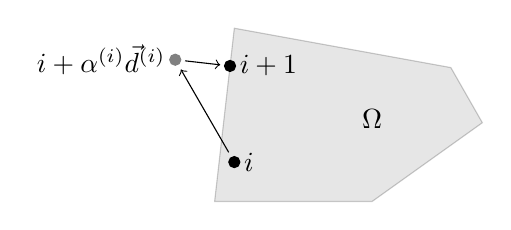
\begin{tikzpicture}
        \draw [thin, draw=black, fill=gray, opacity=0.2] (0,0) -- (.25,2.2) -- (3,1.7) -- (3.4,1) -- (2,0) -- cycle;
        \node [anchor=west] at (.25,.5) {$\mlei{i}$};
        \node (a) at (.25,.5){};
        \filldraw[black] (.25,.5) circle (2pt);
        \node [anchor=east] at (-.5,1.8) {$\mlei{i} + \alpha^{(i)} \vec{d}^{(i)}$};
        \node (b) at (-.5, 1.8){};
        \filldraw[gray] (-.5, 1.8) circle (2pt);
        \node (c) at (0.195563, 1.72096) {};
        \filldraw[black] (0.195563, 1.72096) circle (2pt);
        \node [anchor=west] at (0.195563, 1.72096) {$\mlei{i+1}$};
        \node at (2, 1.05) {$\mathlarger{\mathlarger{\Omega}}$};
        \draw[->] (b) to (c);
        \draw[->] (a) to (b);
    \end{tikzpicture}
\end{figure}

In \cref{alg:mle_search}, $\vec{d}^{(i)}$ is a unit vector denoting a \emph{promising} direction in which to search for a better solution than $\mlei{i}$. The Fisher scoring algorithm is a slight variation of Newton-Raphson\footnote{If the \emph{observed} information matrix is used instead of the \emph{expected} information matrix, the Fisher scoring algortihm is equivalent to Newton-Raphson.} in which
\begin{equation}
    \vec{d}^{(i)} = \infomatrx^{-1}\left(\mlei{i} \right) \score\left( \mlei{i} \right)\,.
\end{equation}
The scalar $\alpha^{(i)} > 0$ is the distance to move from point $\mlei{i}$ to generate the next point, $\mlei{i+1}$. Most naturally, the solution to
\begin{equation}
    \alpha^{(i)} = \argmax_{\alpha > 0} \ell(\mlei{i} + \alpha \cdot \vec{d}^{(i)})    
\end{equation}
is desired, e.g., using \emph{Golden Section} line search to find an approximate solution. Finally, the iterations are repeated until some \emph{stopping criteria} is satisfied. Most naturally, this is given by
\begin{equation}
    \| \score(\mlei{i}) \| < \epsilon\,,
\end{equation}
signifying a stationary point has been reached.

\chapter{General joint distribution}
\label{appendix:generalized_general_joint_likelihood_cand}
By the axioms of probability, the joint distribution of $\rvcand$, $\sv$, $\RV{W}$, and $\RV{A}$ may be decomposed into the chain
\begin{equation}
\begin{split}
\pdf_{\rvcand, \sv, \RV{W}, \RV{A}}(\cand, t, w, \alpha \Given \tparam\sysparamvec) &=\\ &\!\!\!\!\!\!\pmf_{\rvcand \Given \sv, \RV{W}, \RV{A}}(\cand \Given t, w, \alpha, \tparam\sysparamvec) \pmf_{\RV{W}, \RV{A} \Given \sv}(w, \alpha \Given t, \tparam\sysparam) \spdf(t \Given \tparam\sysparam)\,.
\end{split}
\end{equation}

If we remove \cref{asm:?}, the distribution of $\RV{W}$ and $\RV{A}$ may be dependent on $\sv$ but we still they do not carry information about the true parameter index $\tparam\sysparamvec$, thus we may rewrite the above equation as
\begin{equation}
\pdf_{\rvcand, \sv, \RV{W}, \RV{A}}(\cand, t, w, \alpha \Given \tparam\sysparamvec) = \pmf_{\rvcand \Given \sv, \RV{W}, \RV{A}}(\cand \Given t, w, \alpha, \tparam\sysparamvec) \pmf_{\RV{W}, \RV{A} \Given \sv}(w, \alpha \Given t) \spdf(t \Given \tparam\sysparamvec)\,.
\end{equation}

Since $\RV{W}$ and $\RV{A}$ carry no information about the true parameter index $\tparam\sysparamvec$, the maximum likelihood estimate $\mleu$ is independent of the distribution of $\RV{W}$ and $\RV{A}$.
\begin{proof}
\begin{equation}
\begin{split}
    \mleu &= \argmax_{\sysparamvec}
        \ell_n(\sysparamvec)\\
        &= \argmax_{\sysparamvec} \Biggl[ \sum_{i=1}^{n}
        \ln \pmf_{\rvcand \Given \sv, \RV{W}, \RV{A}}(\cand_i \Given t_i, w_i, \alpha_i, \sysparamvec)\\
        &\qquad+ \sum_{i=1}^{n} \ln \spdf(t_i \Given \sysparamvec) + \underbrace{\sum_{i=1}^{n} \ln \pmf_{\RV{W}, \RV{A} \Given \sv}(w_i, \alpha_i \Given t_i)}_{\text{constant}}\Biggr]\,,
\end{split}
\end{equation}
where $w_i = \Card{\cand_i}$ and the last term is constant with respect to $\sysparamvec$ and thus may be dropped from the maximum likelihood equation without changing the point that maximizes the likelihood.
\end{proof}

The sampling distribution of $\mleu$ is a function of $\mfs$ (as opposed to a particular realization), and since $\mfs$ is a function of $\RV{W}$ and $\RV{A}$, the sampling distribution of $\mleu$ is also a function of $\RV{W}$ and $\RV{A}$.

Given a statistical model, the asymptotic sampling distribution of the maximum likelihood estimator is nearly automatic. The most taxing (and uncertain) part is the \emph{model selection}. Since we may not have much confidence in any particular model of the joint distribution of $\RV{W}$ and $\sv$, the \emph{expected} information matrix is sketchy. In general, the \emph{observed} information matrix is preferred. The sampling distribution of $\mleu$ converges in distribution to a multivariate normal with a mean given by $\tparam\sysparamvec$ and a variance-covariance given by the inverse of the \emph{observed} information matrix, written
\begin{equation}
    \sampdu \xrightarrow{d} \mvn\left(\tparam\sysparamvec, \matrx{J}_{\matrx{n}}^{-1}\!\left(\tparam\sysparamvec\right)\right)\,.
\end{equation}

If an accurate distribution of $\RV{W}$ and $\RV{A}$ given $\sv$ could be constructed such that it is dependent on $\tparam\sysparamvec$, then the distribution of $\RV{W}$ and $\RV{A}$ in a sample carries extra information about $\tparam\sysparamvec$.
A plausible model may depend upon $\entropy(\RV{K} \Given \sv = t)$.

\chapter{Sampling distribution of functions of parameters}
\label{sec:app}
Suppose we have a characteristic of interest $\vecstat \colon \mathbb{R}^{m \cdot q} \mapsto \mathbb{R}^{p}$ that is a function of the parametric model.
The \emph{true} value of the characteristic is given by $\vecstat(\tparam\sysparamvec)$.
By the invariance property of maximum likelihood estimators, if $\mleu$ is the maximum likelihood estimator of $\tparam\sysparamvec$ then $\vecstat(\mleu)$ is the maximum likelihood estimator of $\vecstat(\tparam\sysparamvec)$.

By \cref{def:converge_in_dist}, $\sampdu$ is a random vector drawn from a multivariate normal distribution,
\begin{equation*}
\sampdu \sim \mvn\left(\tparam\sysparamvec, \var\left[\sampdu\right]\right)\,,
\tag{\text{\ref{eq:converge_in_dist_weighted} revisited}}
\end{equation*}
therefore $\vecstat\left(\sampdu\right)$ is a random vector. Under the regularity conditions (see \cref{def:reg_cond}), $\vecstat\left(\sampdu\right)$ is asymptotically normally distributed with a mean given by $\vecstat(\tparam\sysparamvec)$ and a variance-covariance given by $\var\left[\vecstat(\sampdu)\right]$, written
\begin{equation}
\vecstat\left(\sampdu\right) \xrightarrow{d} \mvn\left(\vecstat\left(\tparam\sysparamvec\right), \var\left[\vecstat(\sampdu)\right]\right)\,.
\end{equation}

The generative model may be used to generate samples of statistics that are functions of the true parameter index $\tparam\sysparamvec$.
A sample drawn from $\vecstat(\sampdu)$ may be generated by drawing $r$ maximum likelihood estimates from the sampling distribution
\begin{equation}
\Tuple{\mleui{1}, \ldots, \mleui{r}}\,,
\end{equation}
and applying $\vecstat$ to each, resulting in the sample
\begin{equation}
\label{eq:phi_sample}
\Tuple{
\vecstat\left(\mleui{1}\right),
\ldots,
\vecstat\left(\mleui{r}\right)}\,.
\end{equation}
An estimate of the variance-covariance $\var\left[\vecstat(\sampdu\right]$ is given by the sample covariance
\begin{equation}
\begin{split}
\estimator{\var}\left[\vecstat\left(\sampdu\right)\right] &=\\
& \!\!\!\! \frac{1}{r} \sum_{i=1}^{r}
\left(\vecstat\left(\mleui{i}\right) - \vecstat(\mleu)\right)
\left(\vecstat\left(\mleui{i}\right) - \vecstat(\mleu)\right)^\intercal\,.
\end{split}
\end{equation}
Thus,
\begin{equation}
\vecstat\left(\sampdu\right) \sim \mvn\left(\vecstat\left(\mleu\right), \estimator{\var}\left[\sampdu\right] \right)\,.
\end{equation}


\chapter{Bootstrap of sample covariance}
Another estimator of the variance-covariance of $\sampdu$ is given by the sample covariance.
\begin{definition}
	Given a sample of $r$ maximum likelihood estimates, $\mleui{1}, \ldots, \mleui{r}$, the maximum likelihood estimator of the variance-covariance of the sampling distribution of $\mleu$ is given by the sample covariance,
	\begin{align}
	\label{eq:sample_var_sampd}
	\estimator{\var}\left[\sampdu\right] = \frac{1}{r}
	\sum_{i=1}^{r}
	\left(\mleui{i} - \tparam\sysparamvec\right) \cdot
	\left(\mleui{i} - \tparam\sysparamvec\right)^{\intercal}\,.
	\end{align}
\end{definition}
The sample covariance depends upon a random sample of maximum likelihood estimates, and thus the sample covariance is a random matrix. However, by the property that maximum likelihood estimators converge in probability to the true value,
\begin{equation}
\estimator\var\left[\sampdu\right] \xrightarrow{P} \var\left[\sampdu\right]\,,
\end{equation}
it follows that
\begin{equation}
\sampdu \xrightarrow{d} \mvn\left(\tparam\sysparamvec, \estimator\var\left[\sampdu\right]\right)\,.
\end{equation}
If only one maximum likelihood estimate is realized, $\sampdu = \mleu$, then 
the sample covariance given by \cref{eq:sample_var_sampdu} cannot be computed. 
In the \emph{parametric Bootstrap}, the sample covariance is approximated by 
using $\mleu$ as an estimate of $\tparam\sysparamvec$ in the generative model 
described by \cref{dummyref}, i.e.,
\begin{equation}
\mleui{1}, \ldots, \mleui{r} \gets \genSampleMLE\left(\mleu\right)\,,
\end{equation}
and the sample covariance of these approximate maximum likelihood estimates is an asymptotically unbiased estimator of $\var\left[\sampdu\right]$.

\begin{algorithm}
	\DontPrintSemicolon
	\KwIn{\\
		$\qquad \mleu$, an estimate of $\tparam\sysparamvec$.
	}
	\KwOut{\\
		$\qquad$sample covariance of a bootstrapped sample of maximum likelihood estimates.
	}
	\BlankLine
	\SetKwProg{func}{Model}{}{}
	\func{BoostrapCovariance}{$(\mleu)$}
	{
		\For{$i=1$ to $r$}
		{
			$\mleui{i} \gets \genSampleMLE(\mleu)$\;
		}
		\KwRet{sample covariance of $\mleui{1},\,\ldots\,,\mleui{r}$}
	}
	\caption{Sample covariance of a bootstrapped sample of maximum likelihood estimates.}
	\label{alg:samp_du_gen_model}
\end{algorithm}



\end{document}
